\section{Runtime View}


\textcolor{gray}{TO DO LIST (the \textcolor{green} {green} ones can go in the same sequence. the \textcolor{orange}{orange} ones are done)
\begin{enumerate}
    \item \textcolor{orange}{farmer registers SERVICE: authentication - email API: Google}
    \item \textcolor{orange}{farmer logs in SERVICE: authentication + farmer visualizes relevant information (weather conditions and visits) SERVICE: weather conditions - visit API: weather, moisture}
    \textcolor{green}{
    \item farmer make a help request (+notification of new help request received to agronomist) SERVICE: help request (farmer) - notification
    \item agronomist replies to help request (+notification of new help response received to farmer) SERVICE: help request (agronomist) - notification
    \item farmer solves a help request SERVICE: help Request (farmer)}
    \item farmer insert data (+retreive data and computation performance score) SERVICE: harvest service API: moisture, irrigation
    \item agronomist visualizes maps and table in the homepage SERVICE: map - table API: google maps
    \item policy maker visualizes maps and table in the homepage SERVICE: map - time chart API: google maps
    \textcolor{green}{
    \item agronomist updates daily plan (+ notification to farmer) SERVICE: Daily Plan + notification
    \item agronomist confirms daily plan SERVICE: Daily Plan }
    \item agronomist visualizes weather forecasts SERVICE: weather forecasts API: google maps, weather, soil moisture 
    \textcolor{green}{
    \item farmer opens a thread on discussion forum SERVICE: discussion forum
    \item farmer replies to a thread on the discussion forum (+ notification of new post received to farmer who made the thread) SERVICE: discussion forum}
    \item system sends suggestions to farmer (they depend on performance, weather and moisture) SERVICE: suggestion (for the computation) + notification API: weather - moisture
\end{enumerate}
}

\paragraph{Farmer Registration}
\begin{center}
\begin{figure}[H]
\centering
    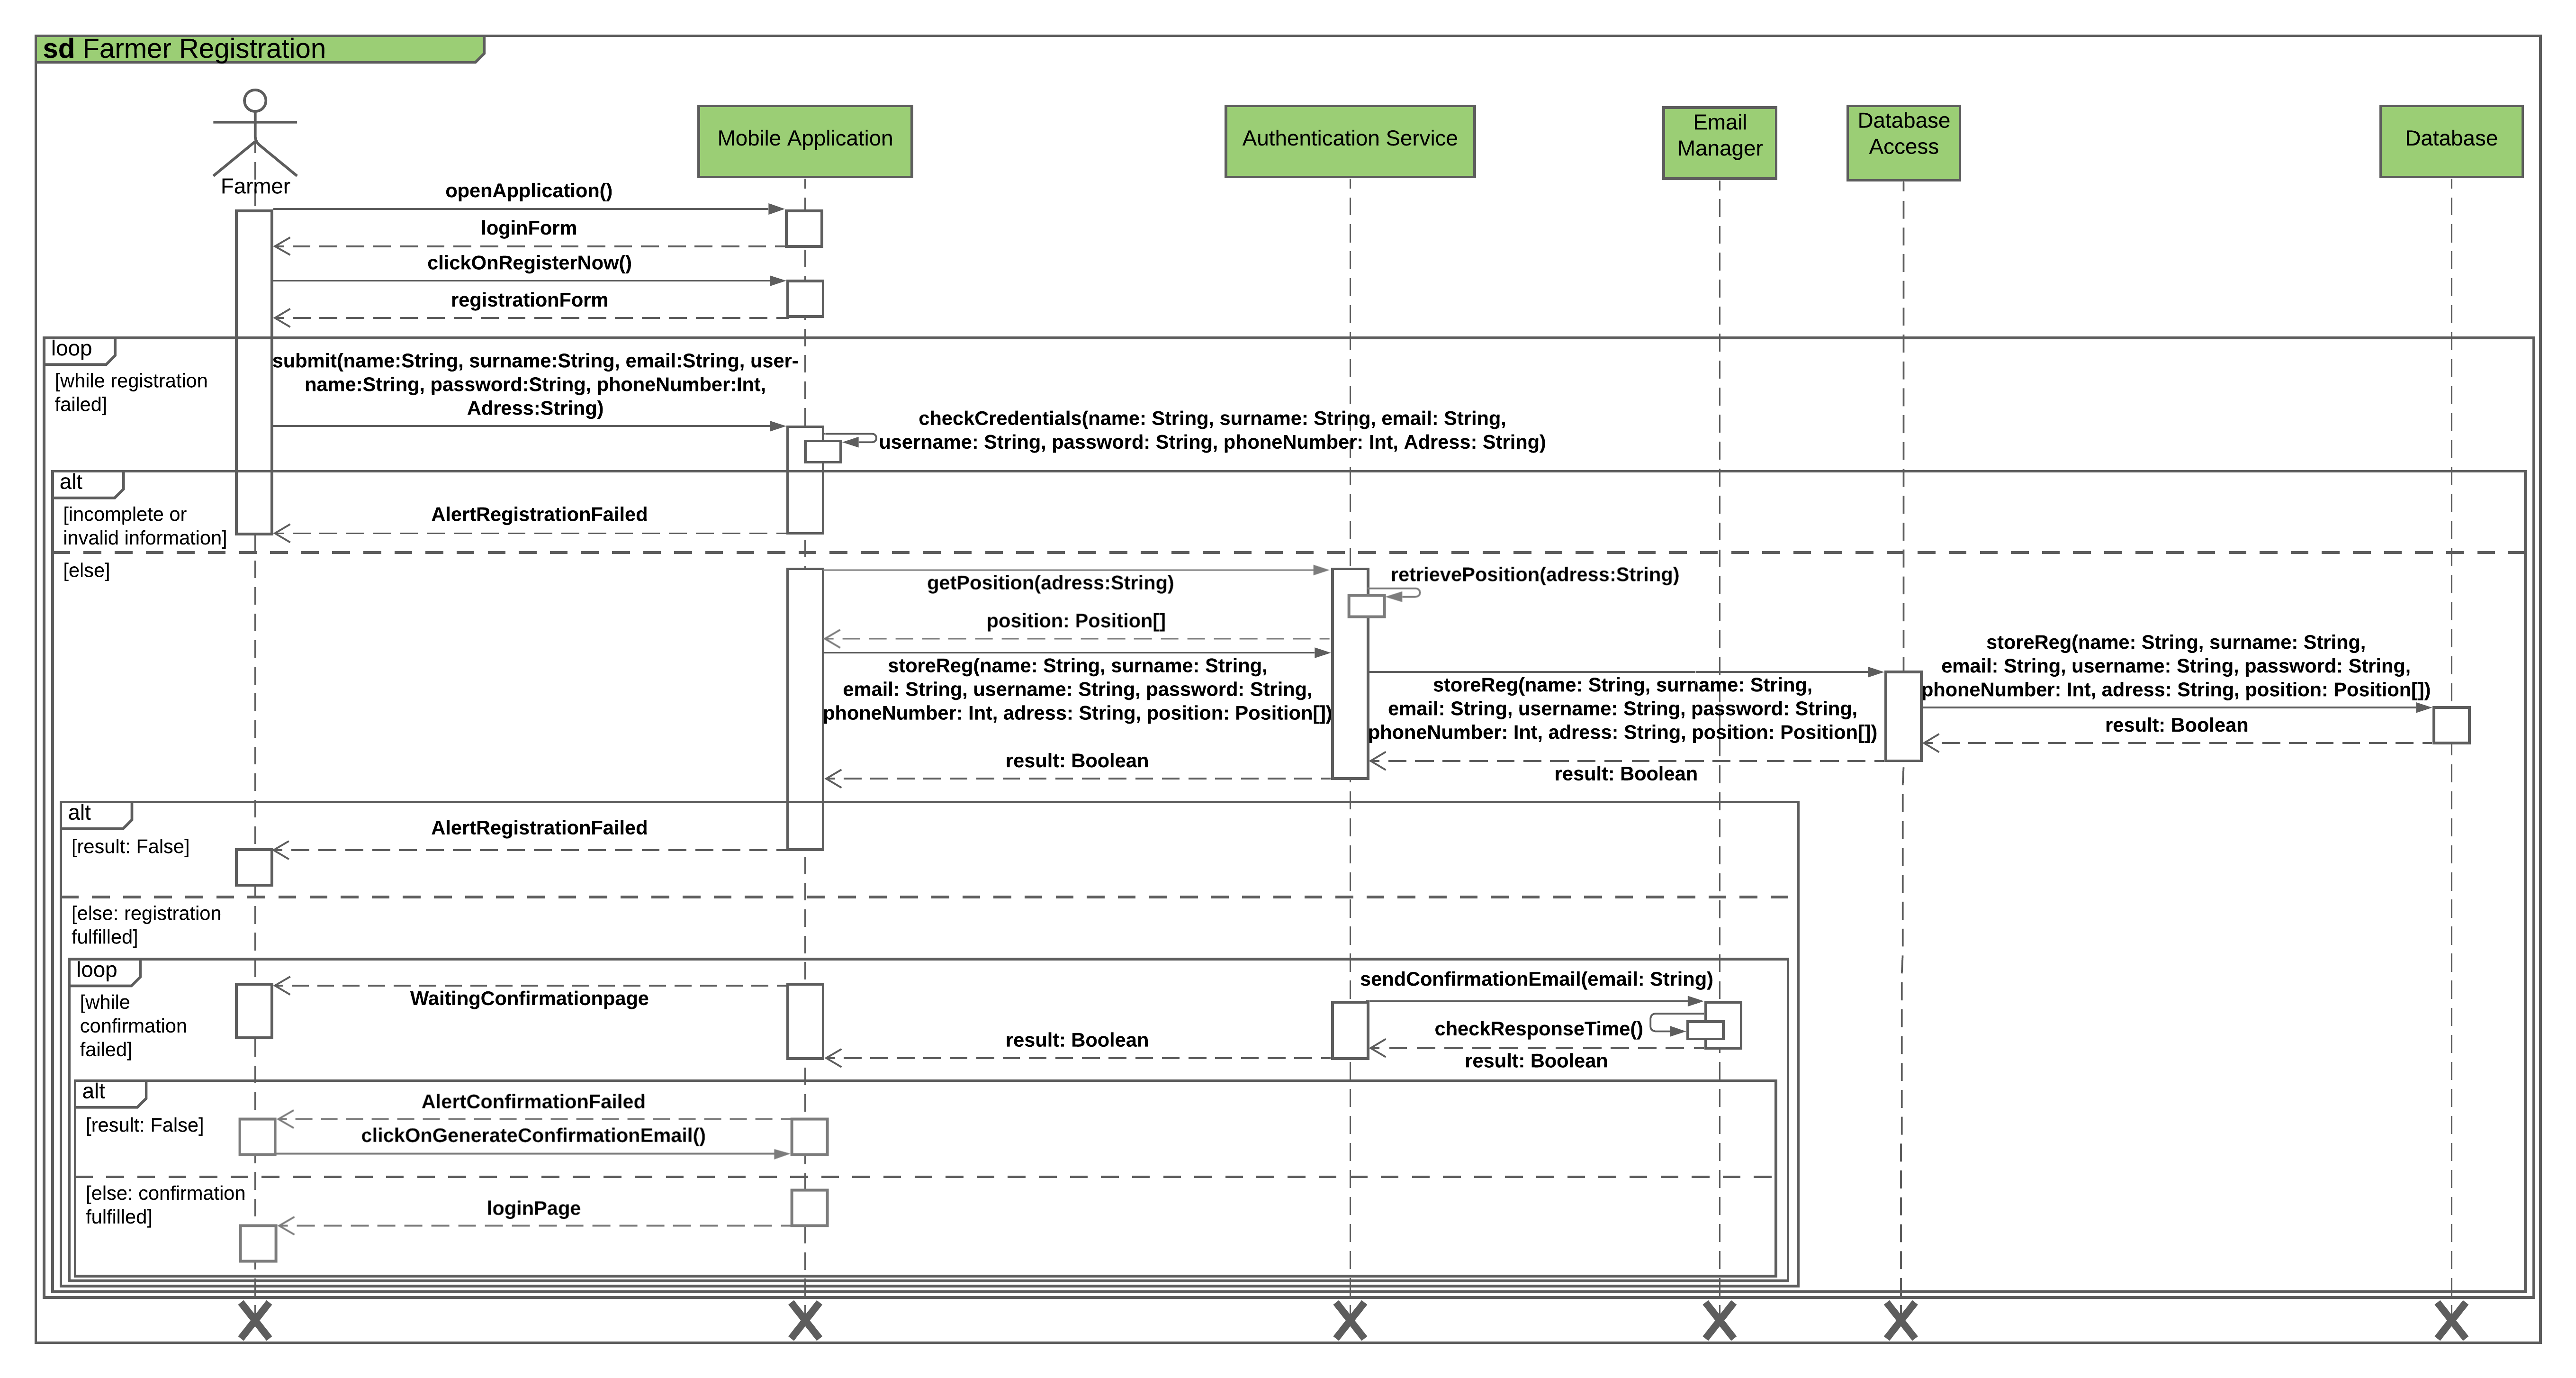
\includegraphics[angle=90,scale= 0.108]{./Images/Farmer Registration Sequence Diagram.png}
    \caption{Farmer Registration Sequence Diagram}
    \label{fig:LandscapeFigure}
\end{figure}
\end{center}

\paragraph{Farmer Login}
\begin{center}
\begin{figure}[H]
\centering
    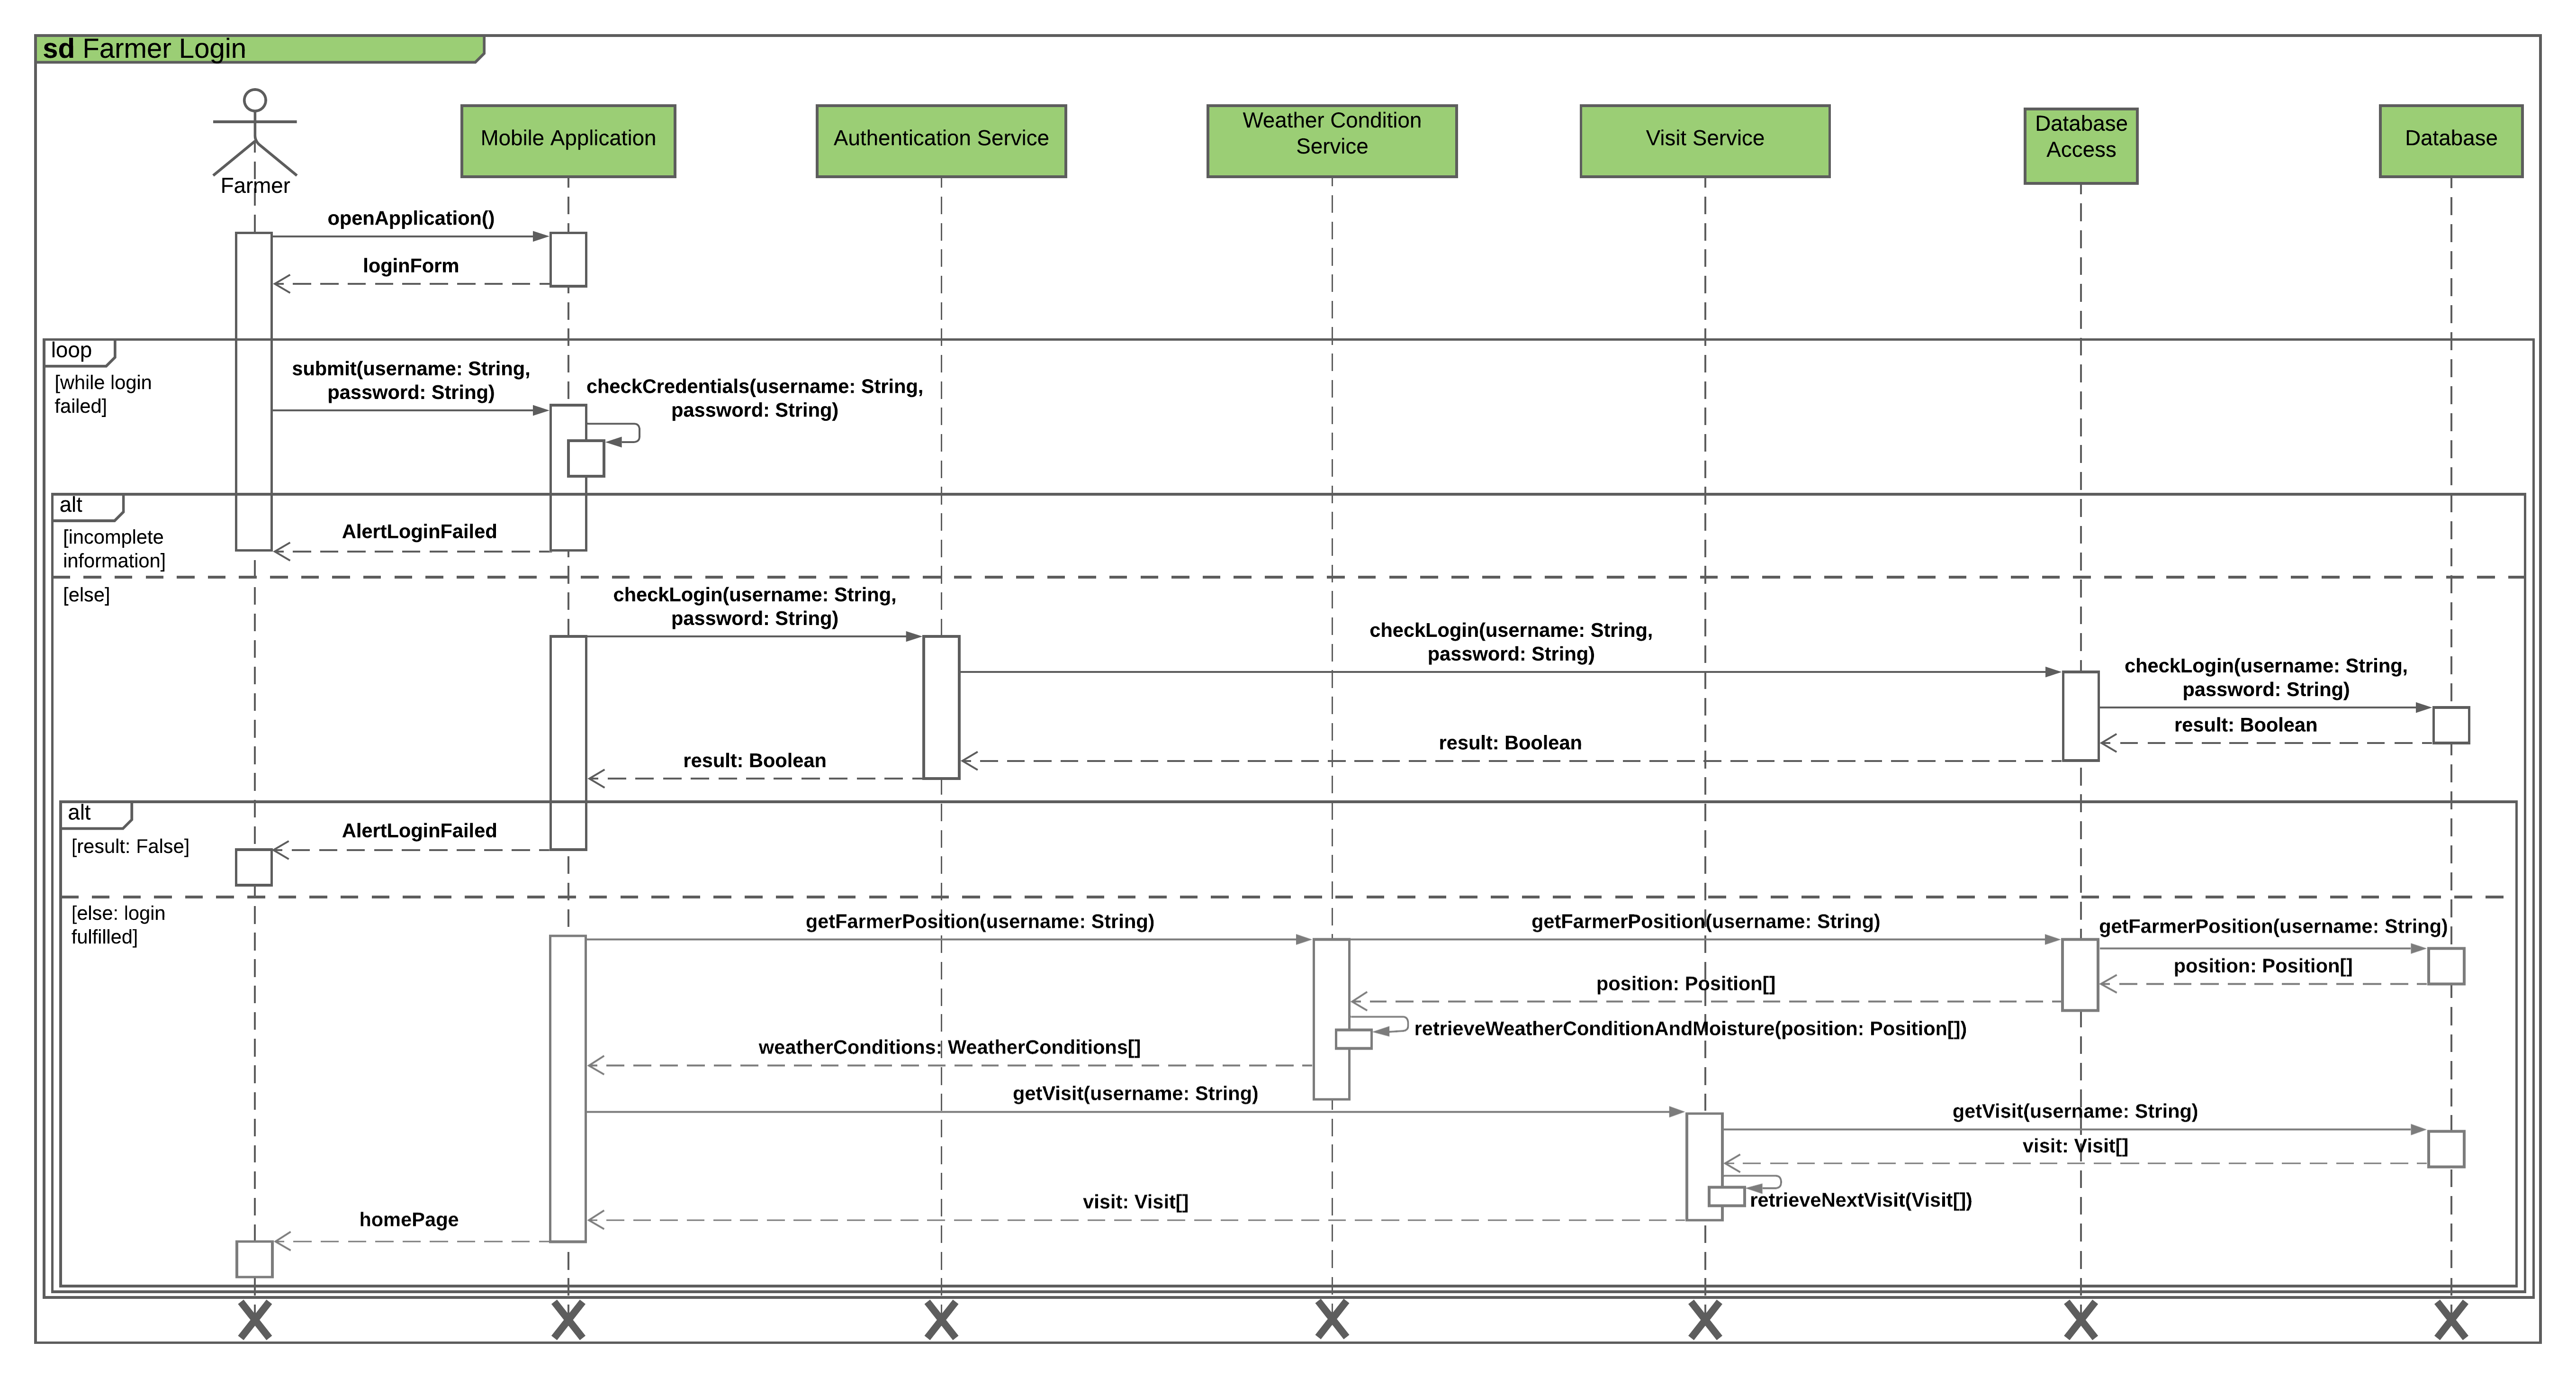
\includegraphics[angle=90,scale= 0.108]{./Images/Farmer Login Sequence Diagram.png}
    \caption{Farmer Login Sequence Diagram}
    \label{fig:LandscapeFigure}
\end{figure}
\end{center}